\chapter{Подготовка к проведению конкурса}

\section{Составление схемы рассадки участников}
После согласования окончательного списка участников мероприятия, был составлен план рассадки конкурсантов в соответствии с их техническими требованиями для демонстрации работ.

На рис.~\ref{img:1} показана составленная рассадка конкурсантов.

\begin{table}[h!]
  \centering
  \begin{tabular}{p{1\linewidth}}
    \centering
    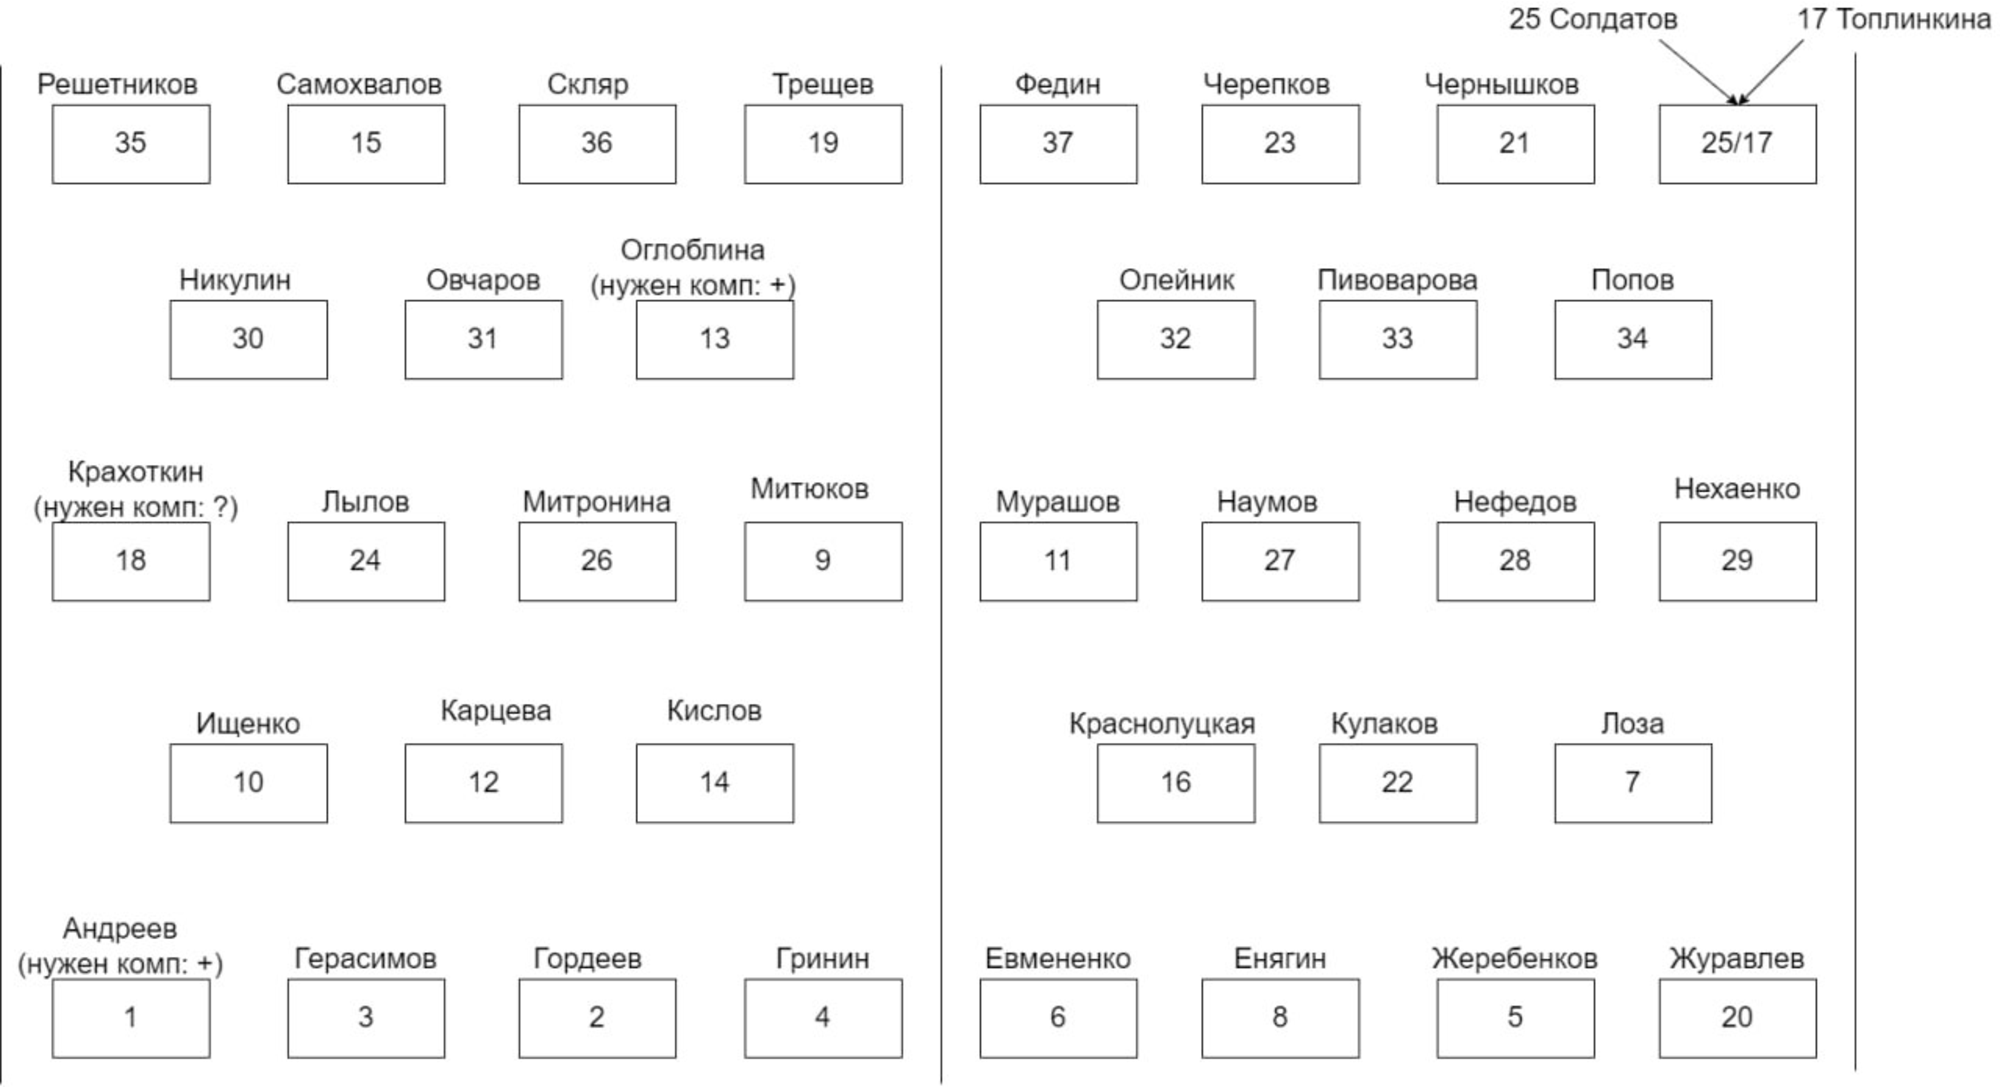
\includegraphics[width=1\linewidth]{./images/places.pdf}
    \captionof{figure}{Cхема рассадки участников}
    \label{img:1}
  \end{tabular}
\end{table}

\section{Установка необходимого ПО}
В процессе подготовки аудитории к проведению конкурса «Шаг в будущее» потребовалось установить необходимое участникам ПО. Для этого был опрошен каждый участник, в результате чего для нуждающихся в стационарном компьютере участвующих было установлено необходимое программное обеспечение для демонстрации работы их проектов.

В процессе опроса был определен следующий список необходимых языков программирования для проектов участников конкурса.

\begin{enumerate}
	\item Python.
	\item C\#.
	\item C++.
	\item JavaScript.
\end{enumerate}

Стационарные компьютеры были проверены на работоспособность. После чего на компьютерах было установлено необходимое ПО. Многие участники конкурса принесли собственные электронные устройства с установленным необходимым программным обеспечением.

\section{Обзвон участников}

За несколько дней до очного тура, был проведен обзвон участников программного салона. С каждого конкурсанта была получена информация о том, приедет ли конкурсант на очный тур, или будет участвовать дистанционно, будет ли компьютер с собой или нужно настроить компьютер в аудитории. 

Кроме того, до каждого конкурсанта была донесена информация о порядке проведения салона, месте и времени проведения очного тура.

\section{Рецензирование участников}

Перед проведением очного тура олимпиады было произведено рецензирование работ участников на основе высланных РПЗ. Пример полученной рецензии приведен на рис.~\ref{img:2}.

\newpage

\begin{table}[h!]
  \centering
  \begin{tabular}{p{1\linewidth}}
    \centering
    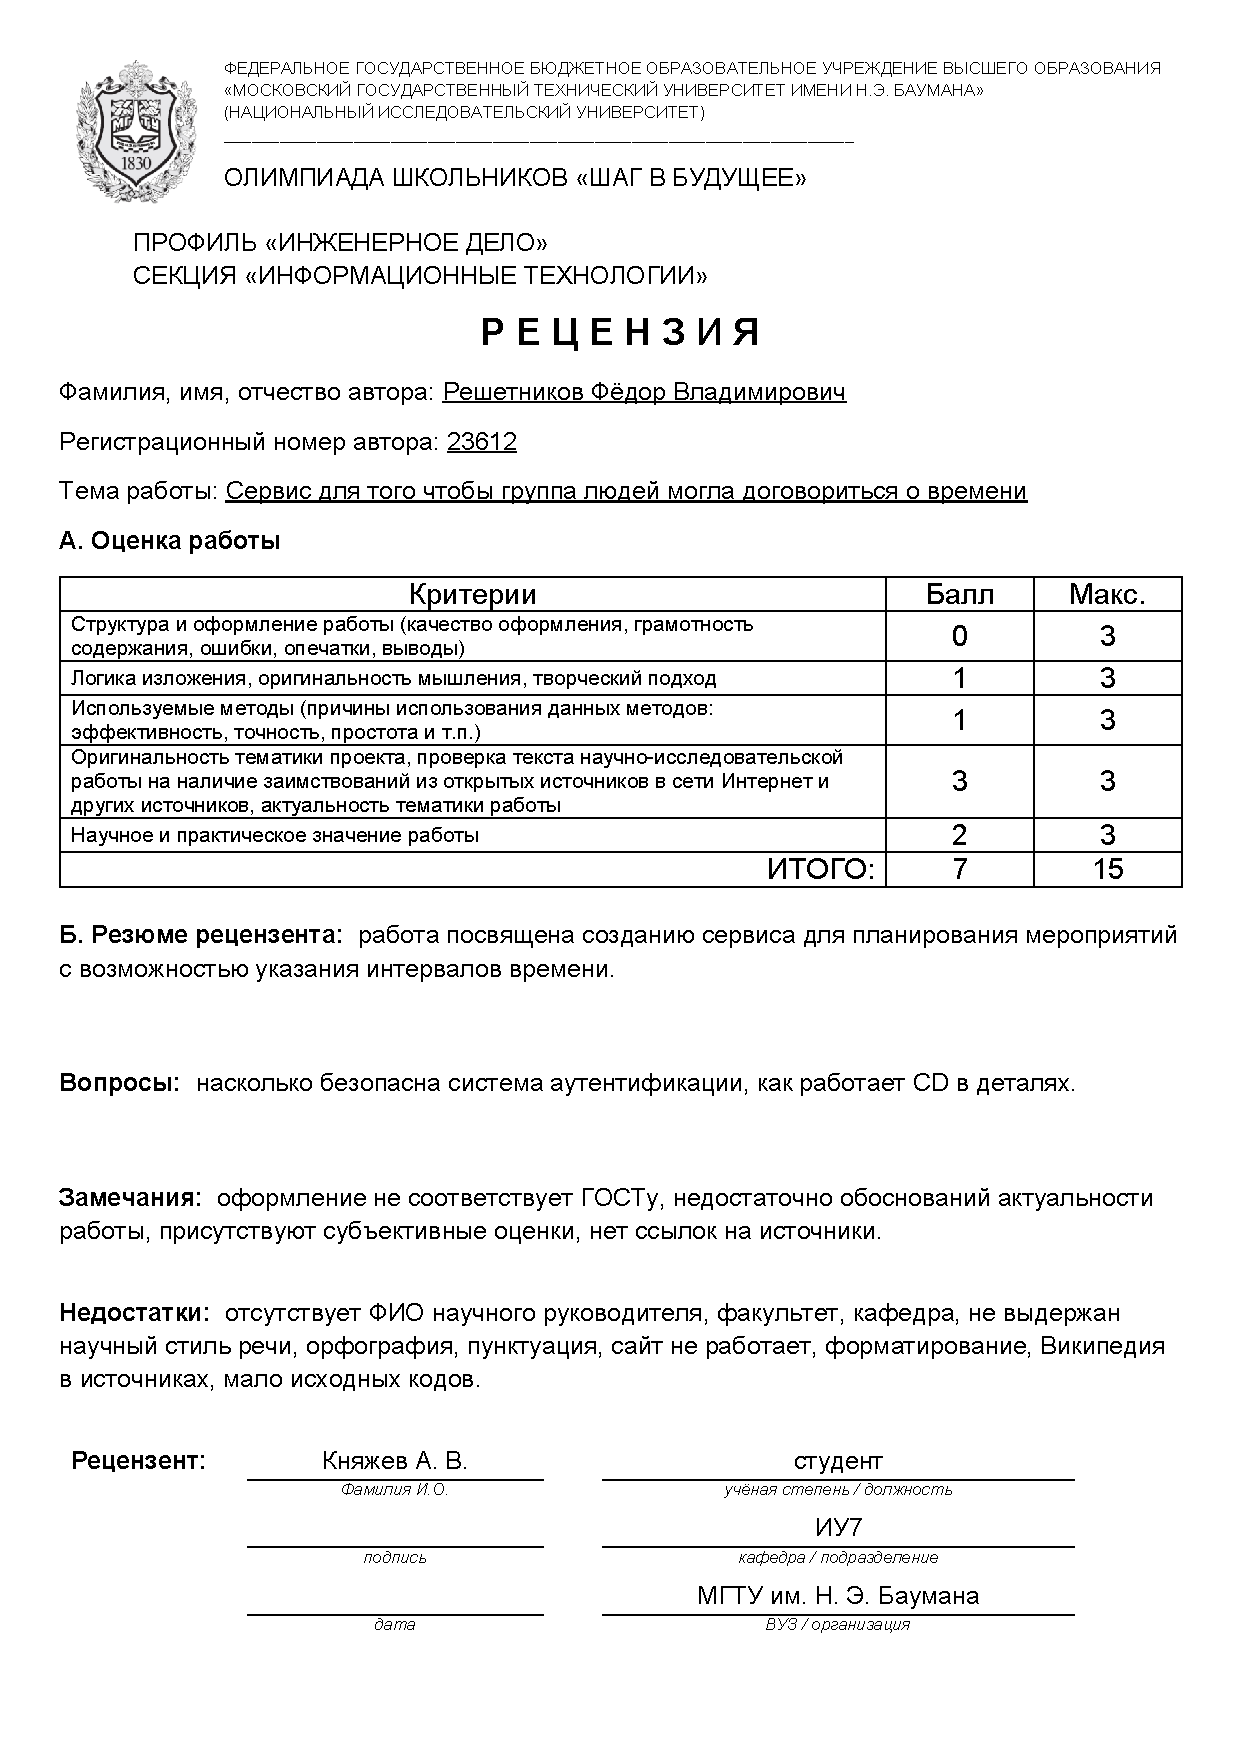
\includegraphics[width=0.9\linewidth]{./images/work.pdf}
    \captionof{figure}{Рецензия}
    \label{img:2}
  \end{tabular}
\end{table}


















 
